% Options for packages loaded elsewhere
\PassOptionsToPackage{unicode}{hyperref}
\PassOptionsToPackage{hyphens}{url}
\PassOptionsToPackage{dvipsnames,svgnames,x11names}{xcolor}
%
\documentclass[
  10pt,
  letterpaper,
  DIV=11,
  numbers=noendperiod]{scrartcl}

\usepackage{amsmath,amssymb}
\usepackage{lmodern}
\usepackage{iftex}
\ifPDFTeX
  \usepackage[T1]{fontenc}
  \usepackage[utf8]{inputenc}
  \usepackage{textcomp} % provide euro and other symbols
\else % if luatex or xetex
  \usepackage{unicode-math}
  \defaultfontfeatures{Scale=MatchLowercase}
  \defaultfontfeatures[\rmfamily]{Ligatures=TeX,Scale=1}
  \setmainfont[]{Helvetica}
\fi
% Use upquote if available, for straight quotes in verbatim environments
\IfFileExists{upquote.sty}{\usepackage{upquote}}{}
\IfFileExists{microtype.sty}{% use microtype if available
  \usepackage[]{microtype}
  \UseMicrotypeSet[protrusion]{basicmath} % disable protrusion for tt fonts
}{}
\makeatletter
\@ifundefined{KOMAClassName}{% if non-KOMA class
  \IfFileExists{parskip.sty}{%
    \usepackage{parskip}
  }{% else
    \setlength{\parindent}{0pt}
    \setlength{\parskip}{6pt plus 2pt minus 1pt}}
}{% if KOMA class
  \KOMAoptions{parskip=half}}
\makeatother
\usepackage{xcolor}
\setlength{\emergencystretch}{3em} % prevent overfull lines
\setcounter{secnumdepth}{5}
% Make \paragraph and \subparagraph free-standing
\ifx\paragraph\undefined\else
  \let\oldparagraph\paragraph
  \renewcommand{\paragraph}[1]{\oldparagraph{#1}\mbox{}}
\fi
\ifx\subparagraph\undefined\else
  \let\oldsubparagraph\subparagraph
  \renewcommand{\subparagraph}[1]{\oldsubparagraph{#1}\mbox{}}
\fi


\providecommand{\tightlist}{%
  \setlength{\itemsep}{0pt}\setlength{\parskip}{0pt}}\usepackage{longtable,booktabs,array}
\usepackage{calc} % for calculating minipage widths
% Correct order of tables after \paragraph or \subparagraph
\usepackage{etoolbox}
\makeatletter
\patchcmd\longtable{\par}{\if@noskipsec\mbox{}\fi\par}{}{}
\makeatother
% Allow footnotes in longtable head/foot
\IfFileExists{footnotehyper.sty}{\usepackage{footnotehyper}}{\usepackage{footnote}}
\makesavenoteenv{longtable}
\usepackage{graphicx}
\makeatletter
\def\maxwidth{\ifdim\Gin@nat@width>\linewidth\linewidth\else\Gin@nat@width\fi}
\def\maxheight{\ifdim\Gin@nat@height>\textheight\textheight\else\Gin@nat@height\fi}
\makeatother
% Scale images if necessary, so that they will not overflow the page
% margins by default, and it is still possible to overwrite the defaults
% using explicit options in \includegraphics[width, height, ...]{}
\setkeys{Gin}{width=\maxwidth,height=\maxheight,keepaspectratio}
% Set default figure placement to htbp
\makeatletter
\def\fps@figure{htbp}
\makeatother
\newlength{\cslhangindent}
\setlength{\cslhangindent}{1.5em}
\newlength{\csllabelwidth}
\setlength{\csllabelwidth}{3em}
\newlength{\cslentryspacingunit} % times entry-spacing
\setlength{\cslentryspacingunit}{\parskip}
\newenvironment{CSLReferences}[2] % #1 hanging-ident, #2 entry spacing
 {% don't indent paragraphs
  \setlength{\parindent}{0pt}
  % turn on hanging indent if param 1 is 1
  \ifodd #1
  \let\oldpar\par
  \def\par{\hangindent=\cslhangindent\oldpar}
  \fi
  % set entry spacing
  \setlength{\parskip}{#2\cslentryspacingunit}
 }%
 {}
\usepackage{calc}
\newcommand{\CSLBlock}[1]{#1\hfill\break}
\newcommand{\CSLLeftMargin}[1]{\parbox[t]{\csllabelwidth}{#1}}
\newcommand{\CSLRightInline}[1]{\parbox[t]{\linewidth - \csllabelwidth}{#1}\break}
\newcommand{\CSLIndent}[1]{\hspace{\cslhangindent}#1}

\KOMAoption{captions}{tableheading}
\makeatletter
\makeatother
\makeatletter
\makeatother
\makeatletter
\@ifpackageloaded{caption}{}{\usepackage{caption}}
\AtBeginDocument{%
\ifdefined\contentsname
  \renewcommand*\contentsname{Table of contents}
\else
  \newcommand\contentsname{Table of contents}
\fi
\ifdefined\listfigurename
  \renewcommand*\listfigurename{List of Figures}
\else
  \newcommand\listfigurename{List of Figures}
\fi
\ifdefined\listtablename
  \renewcommand*\listtablename{List of Tables}
\else
  \newcommand\listtablename{List of Tables}
\fi
\ifdefined\figurename
  \renewcommand*\figurename{Figure}
\else
  \newcommand\figurename{Figure}
\fi
\ifdefined\tablename
  \renewcommand*\tablename{Table}
\else
  \newcommand\tablename{Table}
\fi
}
\@ifpackageloaded{float}{}{\usepackage{float}}
\floatstyle{ruled}
\@ifundefined{c@chapter}{\newfloat{codelisting}{h}{lop}}{\newfloat{codelisting}{h}{lop}[chapter]}
\floatname{codelisting}{Listing}
\newcommand*\listoflistings{\listof{codelisting}{List of Listings}}
\makeatother
\makeatletter
\@ifpackageloaded{caption}{}{\usepackage{caption}}
\@ifpackageloaded{subcaption}{}{\usepackage{subcaption}}
\makeatother
\makeatletter
\@ifpackageloaded{tcolorbox}{}{\usepackage[many]{tcolorbox}}
\makeatother
\makeatletter
\@ifundefined{shadecolor}{\definecolor{shadecolor}{rgb}{.97, .97, .97}}
\makeatother
\makeatletter
\makeatother
\ifLuaTeX
  \usepackage{selnolig}  % disable illegal ligatures
\fi
\IfFileExists{bookmark.sty}{\usepackage{bookmark}}{\usepackage{hyperref}}
\IfFileExists{xurl.sty}{\usepackage{xurl}}{} % add URL line breaks if available
\urlstyle{same} % disable monospaced font for URLs
\hypersetup{
  pdftitle={Making a case for the use of digital footprint data for evidence-based policies in response to human mobility changes after COVID-19 in Latin America},
  pdfauthor={Francisco Rowe; Carmen Cabrera-Arnau; Miguel González-Leonardo; Andrea Nasuto; Ruth Neville},
  colorlinks=true,
  linkcolor={blue},
  filecolor={Maroon},
  citecolor={Blue},
  urlcolor={Blue},
  pdfcreator={LaTeX via pandoc}}

\title{Making a case for the use of digital footprint data for
evidence-based policies in response to human mobility changes after
COVID-19 in Latin America}
\author{\small Francisco Rowe \and \small Carmen
Cabrera-Arnau \and \small Miguel González-Leonardo \and \small Andrea
Nasuto \and \small Ruth Neville}
\date{}

\begin{document}
\maketitle
\begin{abstract}
\textbf{Abstract}. Text for abstract
\end{abstract}
\ifdefined\Shaded\renewenvironment{Shaded}{\begin{tcolorbox}[boxrule=0pt, borderline west={3pt}{0pt}{shadecolor}, interior hidden, sharp corners, enhanced, breakable, frame hidden]}{\end{tcolorbox}}\fi

\hypertarget{introduction}{%
\section{Introduction}\label{introduction}}

Digital footprint data (DFD) are increasingly becoming a vital component
of the data ecosystem to measure and monitor human mobility. DFD are
digital traces left as a result of social interactions on digital
platforms, such as the Internet through web search engines
(e.g.~Google), social media networks (e.g.~Twitter and Facebook),
commercial systems in the way of transactions (e.g.~payment systems),
sensor networks to capture environmental and human changes (e.g.~fitness
trackers, temperature and sound sensors), and imagery collected via
satellites, cameras, drones, CCTV and imaging devices. Digital traces
encoding location recorded through Call Detail Records (CDRs), eXtended
Detail Records (XDR), Global Positioning System (GPS), Bluetooth and
smart card data have been particularly valuable to reconstruct a
traceable digital representation of human mobility.

These forms of DFD offer three key opportunities to capture human
mobility (1) at higher geographical and temporal granularity; (2) over
extensive geographical coverage comprising entire population systems or
geographical areas; and (3) in real or near-real time {[}REF{]}. These
attributes have enabled to complement traditional data sources to
capture human mobility at various geographically scales, including urban
mobility {[}REF{]}, internal migration {[}REF{]} and international
migration {[}REF{]}

Yet, the use of DFD poses significant challenges. These data are a
by-product of administrative processes. They are not collected for
research purposes. Their use involves major conceptual, methodological,
data and ethical challenges {[}REF{]}. For instance, turning raw DFD
into actionable, usable information requires significant data
engineering, embracing data-driven hypotheses, accounting for data
biases, ensuring privacy and anonymity, and integrating and validating
the resulting outcomes with external data sources {[}REF{]}. These
challenges to be overcome to unleash the opportunities offered by DFD.

An increasing number of ``Data for Good'' initiatives have been
developed to leverage the potential positive social impact of DFD. These
include data governance, data strategy and data sharing initiatives
(European Commission. Joint Research Centre. 2022). Data governance
initiatives involve efforts focused on the provision of guidance about
best practices for the collection, storage, share and use DFD for the
social good. Data strategy initiatives focus on building capacity in
civil society by designing data strategies for nonprofits and government
agencies, such as Data-Pop Alliance and the Open Data Institute. Data
sharing initiatives entail the creation and facilitation of access to
datasets by data providers for organisations seeking to generate data
solutions and positive social impact. These initiatives include
\href{https://dataforgood.facebook.com/dfg/about}{Data for Good at Meta}
and \href{https://www.waze.com/wazeforcities/}{Waze Partner Hub}.

Enabled by these initiatives, the use of DFD seems to have been - much
more promising in less developed countries given data scarcity.

\begin{itemize}
\item
  Discuss how digital footprint data have been used in more developed
  countries or global north
\item
  Highlight the limited use of digital footprint data in the global
  south
\item
  Aim: Use of digital footprint data for mobility and policy response
\item
  Argue case for COVID and mobility
\item
  Discuss the hypotheses we intend to test and our focus on capital
  cities
\item
  Structure
\end{itemize}

\hypertarget{background}{%
\section{Background}\label{background}}

\hypertarget{the-impact-of-covid-19-on-internal-population-movements}{%
\subsection{The impact of COVID-19 on internal population
movements}\label{the-impact-of-covid-19-on-internal-population-movements}}

Globally, there is evidence that the COVID-19 pandemic constrained both
shorth- and long-distance movements within national boundaries
(Nouvellet et al. 2021; González-Leonardo, Rowe, and Fresolone-Caparrós
2022; Wang et al. 2022; Rowe, González-Leonardo, and Champion 2023).
Declines were documented across the Global North during the first year
of the pandemic, in the United States (Ramani and Bloom 2021), some
European countries, Japan and Australia (Rowe, González-Leonardo, and
Champion 2023), from 2.5\% in Spain to 8.5\% in Australia. Drops mostly
occurred when governments implemented non-pharmaceutical interventions,
such as stay-at-home requirements, travel restrictions, mobility
restrictions, business and school closures. Levels of human mobility
within countries, however, recovered pre-pandemic values following the
elimination of lockdowns and other stringency measures. Declines on
human mobility were attributed to lockdowns, increasing teleworking and
restrictions of movements, but also to a loss of labour market dynamism
as a consequence of the economic recession during the pandemic (Perales
and Bernard 2022). In addition to evidence in the Global North, drops in
internal population movements were also found in Latin American,
declining by about 10\% during periods of severe stringency measures
(Aromí et al. 2023). The highest declines occurred in Bolivia, Ecuador
and Argentina, ranging from 16\% to 19\%, while they did not reach 3\%
in Paraguay and Venezuela.

In global north countries, the COVID-19 pandemic also modified the
patters of internal population movements between large cities and areas
with lower population densities (Rowe, González-Leonardo, and Champion
2023). Variations were found in the United States (Ramani and Bloom
2021), United Kingdom (Rowe, González-Leonardo, and Champion 2023; Wang
et al. 2022), Spain (González-Leonardo et al. 2022; González-Leonardo,
Rowe, and Fresolone-Caparrós 2022), Germany (Stawarz et al. 2022),
Sweden (Vogiazides and Kawalerowicz 2022), Norway (Tønnessen 2021),
Australia (Perales and Bernard 2022) and Japan Kotsubo and Nakaya
(2022). Net-migration rates in large cities declined in the United
States, Germany, Norway, Sweden and Japan during 2020, while they
increased in their suburbs. (Ramani and Bloom 2021) called this
phenomenon as ``donut effect'', reflecting a decrease in population
inflows to urban centers (urbanization) and a growth of movements from
cities to their suburban rings (suburbanization). Nonetheless, there is
no evidence of a ``donut effect'' in the United Kingdom, Spain and
Japan, as net-flows in suburbs did not show significant changes.
However, inflows to large cities also declined and counterurbanisation
movements increased, reflecting unusual population gains in rural areas.
In Spain, Sweden, Japan and Germany, holiday town with second homes of
wealthy individuals were also found as popular destination for people
leaving large cities during the pandemic. It suggests that wealthy
populations and professionals who are able to work remotely seems to
underpin movements from large cities to areas with lower population
densities where they own second residences (Haslag and Weagley 2021;
Tønnessen 2021).

Despite the above-mentioned changes to the human mobility system during
the pandemic, research suggests that pre-existing macro-structures of
internal population movement across the rural-urban continuum were not
altered, since the majority of movements continued to occur within and
between urban areas, and changes are not likely to endure (Rowe,
González-Leonardo, and Champion 2023). For instance, mobility patterns
returned to those registered before the pandemic after the lockdown in
the United Kingdom (Rowe et al. 2022; Wang et al. 2022). The pandemic
caused minor impacts on spatial patterns of internal population
movements in Australia, and variations attributed to COVID-19
disappeared in late 2020 (Perales and Bernard 2022). Urbanisation levels
returned to those register prior to the pandemic in Spain when the
lockdown ended in mid-2020 (González-Leonardo et al. 2022), although
unusually high levels of counterurbanisation persisted over 2021,
despite decreasing over the year (González-Leonardo, Rowe, and
Fresolone-Caparrós 2022).

Previous work provided a good understanding on how human mobility across
the rural-urban hierarchy was affected by the pandemic in the Global
North. However, less is known about COVID-19 impacts on movements
between cities, suburbs and rural areas in the Global South and the
durability of potential changes. Anecdotal evidence, based on small
surveys carried out in India (Irudaya Rajan, Sivakumar, and Srinivasan
2020) and South Africa (Ginsburg et al. 2022), pointed out that flows
from large cities to less populated areas increased due to the return of
workers to their hometown, while movements of labour force to cities
decreased. Both surveys saw that the economic downturn caused by
non-pharmaceutical interventions during the pandemic (Ghosh, Seth, and
Tiwary 2020) underpinned declining inflows of workers to cities and
increasing returns among people who lost their jobs. The above-mentioned
anecdotal evidence suggests that vulnerable populations seem to have
played a role in movements to and away from large cities during the
pandemic in the Global South.

Nonetheless, a recent study demonstrated that wealthy individuals from
large cities in Brazil, Colombia, Indonesia, Mexico, Philippines and
South Africa moved to lees populated areas during the first wave of
COVID-19 (Lucchini et al. 2023). On average, residents from high-wealthy
neighborhoods were 1.5 times more likely to leave cities compared to
those from low-wealthy areas. These finding is in line to results in
Global North countries. Despite anecdotal evidence suggesting pandemic
impacts on the patterns of internal population movements across the
rural-urban hierarchy in some Global South countries, lack of data has
not allowed for quantifying the magnitude and durability of potential
impacts on the human mobility system. To fill the gap, we use Facebook
data to analyse the effect of COVID-19 on the patterns of internal
population movements in Argentina, Chile, Colombia and Mexico.

\hypertarget{human-mobility-across-the-rural-urban-continuum-in-latin-american-countries}{%
\subsection{Human mobility across the rural-urban continuum in Latin
American
countries}\label{human-mobility-across-the-rural-urban-continuum-in-latin-american-countries}}

Currently, Latin America has the highest urbanization rate in the world
after North America, totaling 81\% (Nations" 2019). It means that the
population is highly concentrated across space within Latin American
countries, particularly in large cities with more than one million
inhabitants, where half of urban residents are settled (Pinto da Cunha
2002; A. E. Lattes, Rodríguez, and Villa 2017). High urbanization rates
are due to massive levels of population redistribution from rural
settlements to cities until the 1980s, mostly during the fast
industrialisation period from early-1950s to late-1970s, when population
gains were mainly observed in chief cities (Firebaugh 1979; A. Lattes
1995; J. Sobrino 2012). Internal population movements in Latin America
have been declining since the 1980s, as rural population stocks were
depleted (Chávez Galindo et al. 2016) and the industrial crisis leaded
to deconcentration trends in large cities, such as Santiago de Chile
{[}González Ollino and Rodríguez Vignoli (2006)) or Mexico City (Jaime
Sobrino 2006), where long distance inflows have declined. In sum, middle
size cities became more attractive to internal migrants as a consequence
of increasing domestic and foreign investment in export-oriented
industries or tourism activities, leading to geographic economic
dispersal (Brea 2003; Pérez-Campuzano 2013; Chávez Galindo et al. 2016).
Nowadays, movements between cities dominate the internal migratory
system in Latin American countries (Bernard et al. 2017;
Rodríguez-Vignoli and Rowe 2018; Nations" 2019). About 80\% of internal
migrants moved between cities, according to the 2010-11 census round
(Rodríguez-Vignoli and Rowe 2018). Medium-sizes cities from 500.000 to 1
million residents showed the highest population gains by internal
migration, while large cities with more than 1 million residents
registered balanced rates and small cities with less than 500.000
inhabitants lost population by internal mobility (Rodríguez-Vignoli and
Rowe 2018).

Latin American cities have shown a significant growth in terms of land
development in their urban peripheries. Since the 1970s, large cities,
such as Santiago de Chile, Buenos Aires or Mexico City, but also middle
and small cities have experienced suburbanisation (Graizbord and Acuña
2007; Chávez Galindo et al. 2016). Suburbanisation flows comprise
middle- and high-class families moving from cities to auto-segregated
areas in the periphery (Borsdorf 2003; Rodríguez Vignoli and Rowe 2017).
Low-income individuals also settle in slams across suburbs but, in this
case, in those areas where the land cost is cheaper (Janoschka 2002;
Rodríguez Vignoli and Rowe 2017). Both residents in auto-segregated
areas and slams commute daily to cities, mainly for work reasons (Chávez
Galindo et al. 2016). Most recently, reurbanisation trends have been
identified in central areas due to gentrification dynamics, although
suburbanization flows continue to dominate short distance movements (J.
Sobrino 2012; Chávez Galindo et al. 2016). In this repot, we explore
COVID-19 impacts on the patterns of human mobility across the
rural-urban continuum in Latin America.

\hypertarget{data}{%
\section{Data}\label{data}}

\hypertarget{meta-facebook-data}{%
\subsection{Meta-Facebook Data}\label{meta-facebook-data}}

The multinational technology conglomerate Meta offers a range of data
products aimed for social good through their Data for Good programme,
which is open to trusted partners including universities, non-profit
organisations, and international institutions. The data is available at
small spatial and temporal scales and has the potential to improve how
we respond to real-world crises or unusual events, such as earthquakes,
hurricanes, floods or pandemics (Maas et al. 2019). In particular, the
Data for Good programme offers location data, gathered from Facebook app
users who have the Location Services setting turned on on their
smartphone. Meta uses the location data for a wide variety of
applications in addition to the Data for Good programme, including
providing customised services to its users such as finding nearby
friends, providing information about nearby Wi-Fi hotspots, and
location-relevant ads. The collected location data also enables
targeting of AMBER alerts and prompts to check-in as ``safe'' after a
hazard event.

While the raw location data remains available only to the data owners,
the datasets available through Data for Good consist of anonymised and
aggregated near real-time data corresponding to a period of crisis which
might extend over several weeks, months or years. The datasets also
contain historical location data as a baseline period before the event
(Maas et al. 2019).

We analyse human mobility during the COVID-19 pandemic using the
datasets Coronavirus Disease Prevention Map of Facebook Population
During Crisis (Tile Level) and Coronavirus Disease Prevention Map of
Facebook Movements During Crisis (Tile Level), hereinafter Facebook
Population and Facebook Movements datasets. Specifically, we analyse
human movement data from four Latin American countries: Argentina,
Chile, Colombia and Mexico. The former dataset allows us to analyse how
the number of Facebook users changed across space during the COVID-19
pandemic. The focus of our analysis, however, is on the latter, which
contains information about the evolution of spatial patterns of mobility
during COVID-19.

The datasets contain data corresponding to a two-year period, starting
on the 10th March 2020 and ending in mid-March 2022. Data are temporally
aggregated into three 8-hour daily time windows (00:00-08:00,
08:00-16:00 and 16:00-00:00). The datasets also include data for
baseline levels before COVID-19 based on a 45-day period ending on the
10th of March of 2020. The baseline data is computed using an average
for the same time of the day and day of the week in the period preceding
the crisis (e.g., average over all data collected on a Monday from 00:00
to 8:00 or average over all data collected on a Wednesday from 16:00 to
00:00). For more details on how the baseline values are computed, see
(Maas et al. 2019).

The data is spatially aggregated into units called Tiles, according to
the Bing Maps Tile System developed by Microsoft (Microsoft). This
widely-used system offers a variety of world partitions, where the
spatial units are square cells at various levels of resolution. The Data
for Good datasets are typically generated using Bing tile levels 13
through 16, where level 13 results in tiles that are about 4.9 x 4.9 km
at the Equator (Maas et al. 2019).

The Facebook Population data provides the number of mobile app users who
have the Location Services setting turned on, aggregated by tile. The
location of each user in a given 8-hour time window is determined by the
tile where they spent most of the time within that window. The Facebook
Movement data captures the number of mobile app users who have the the
Location Services setting turned on moving between a pairs of tile. The
origin and destination of a movement are defined as the locations where
a user spent most time between two subsequent time windows (e.g.,
00:00-8:00 and 8:00-16:00). In addition to the count data, both the
Facebook Population and the Facebook Movement datasets include the
percentage difference between the number of counts during the crisis
period and the corresponding baseline level for each entry.

Prior to releasing the datasets, information on personal characteristics
of users is removed and several techniques are applied to ensure privacy
and anonymity. Small-count dropping is one of these techniques, whereby
a data entry is removed from the data set if population or movement
counts are lower than 10 during the crisis period, the baseline period
or both. While this technique makes it harder to identify individual
users based on their movement patterns, the removal of data entries
containing locations with small counts may lead to an
underrepresentation of the population in these places. Another of these
techniques consists in adding a small undisclosed amount of random noise
to ensure that it is not possible to ascertain precise, true counts for
sparsely populated locations. In order to produce a smooth population
count surface, spatial smoothing using inverse distance-weighted
averaging is also applied (see (Maas et al. 2019) for details).

\hypertarget{covid-19-stringency-data}{%
\subsection{COVID-19 stringency data}\label{covid-19-stringency-data}}

To understand the patterns of mobility in the context of the COVID-19
pandemic, we use the stringency index as a measure of the level of
nonpharmaceutical interventions to COVID-19, such as social distancing
and lockdowns. The stringency index ranges from 0 to 100, with 100 being
the value corresponding to the most strict scenario. The values for the
stringency index were retrieved from the COVID-19 government response
tracker
(https://www.bsg.ox.ac.uk/research/research-projects/covid-19-government-response-tracker).
For more information, see Hale et al. (Hale et al. 2021).

\hypertarget{worldpop-population-data}{%
\subsection{Worldpop population data}\label{worldpop-population-data}}

An additional data set from WorldPop was used to capture the spatial
distribution of actual population in the different countries analysed
here. The WorlPop poulation dataset is in raster format and contains
gridded population data at 1 sqkm resolution. We processed the WorlPop
population data so it is spatially aggregated according to the Bing Maps
Tile System. The level of detail was chosen so it coincides with that
used in the Facebook Population and the Facebook Movements data for each
of the countries analysed in this study.

\hypertarget{sec-methods}{%
\section{Methods}\label{sec-methods}}

\hypertarget{sec-methods1}{%
\subsection{Population density classification}\label{sec-methods1}}

In this study, we aim to understand how the population density at the
origin and destination locations might influence mobility behaviours. To
help characterise the population density of different locations, we
consider the Worldpop population data aggregated into Bing tiles. We
then use the Jenks natural breaks classification method in order to
obtain 10 categories of population density, with categories 1 and 10
being the least and most dense categories respectively. This
categorisation of Bing tiles, which offers a greater level of detail
than the traditional binary rural/urban classification, is represented
in Figure~\ref{fig-map}. In the Figure, we have included maps for the
four countries in the study showing the Bing tiles coloured according to
the population density category they belong to. It is possible to see
from the in-set histograms that Argentina and Chile have very skewed
distributions due to the strong concentration of highest-density areas
in just a few tiles belonging to their capital cities, Buenos Aires and
Santiago. By contrast, Colombia and Mexico display more balanced
population density distributions across tiles. It is important to note
that the cut-off values for each population density category vary across
countries, but we expect tiles belonging to the same category in each
country to have similar functions in the urban hierarchy (e.g.~the
high-density tiles belonging to category 10 always correspond to major
urban centres that act as socioeconomic hubs in their respective
regions).

\begin{figure}

{\centering 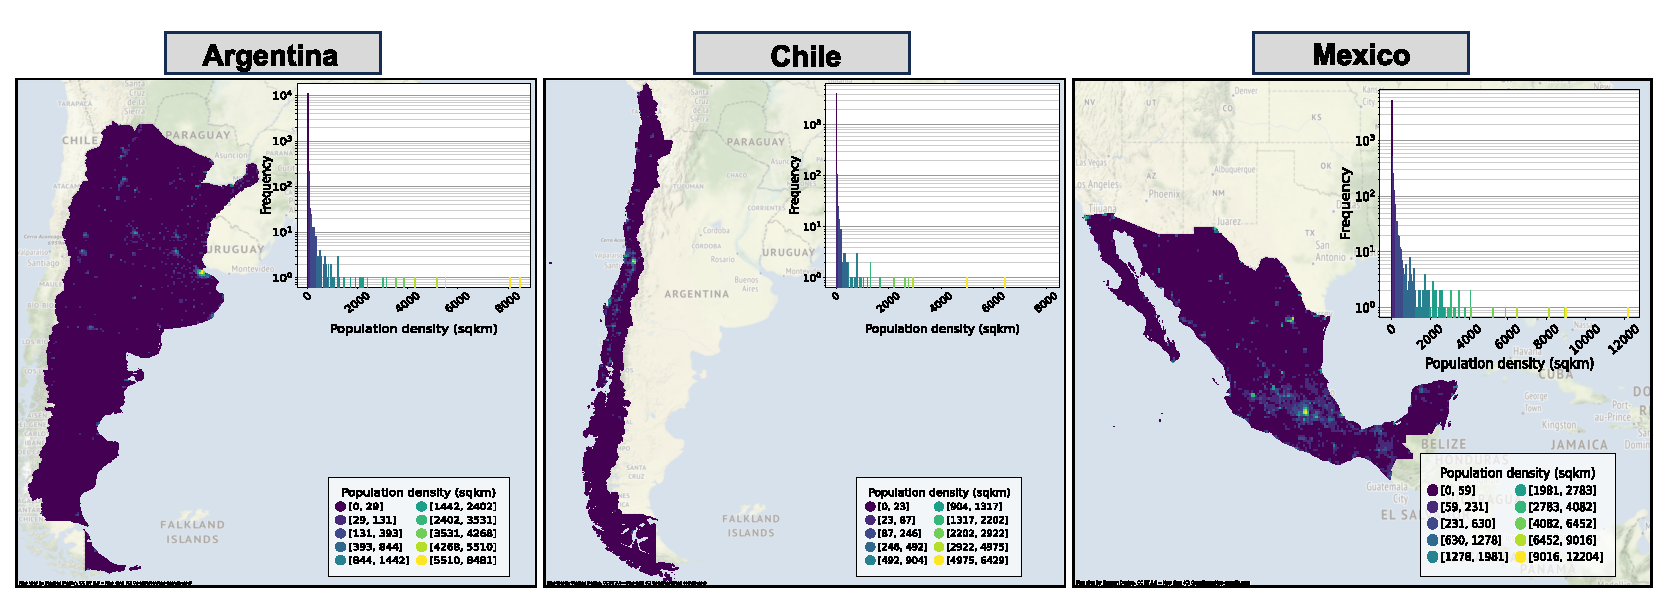
\includegraphics{./outputs/Map_density_histogram_minus_Colombia.pdf}

}

\caption{\label{fig-map}Population density at Microsoft Bing tile level,
Argentina, Chile and Mexico.}

\end{figure}

In order to provide a better intuition of the type of areas that each
population density category represents, we also include
(\textbf{tab-places?}), where we give a few examples of names of places
belonging to each density category.

{[}Table{]}\{\#tab-places\}

\hypertarget{tile-based-mobility-metrics}{%
\subsection{Tile-based mobility
metrics}\label{tile-based-mobility-metrics}}

We measured changes in the intensity of movement by computing the
variation in the number of inflows and outflows by population density
category, i.e.~the number of people entering and leaving tiles belonging
to a specific population density category. We did this across all tiles
of Argentina, Chile, Colombia and Mexico for two distinctive months
during the course of the COVID-19 pandemic: May 2020 and March 2022.
Specifically, we use the percentage change in the intensity of a
population flow as provided in the Facebook Movement data sets (Maas et
al. 2019). For each entry in the dataset, which represents a flow of
people between an origin and a destination tile, the percentage change
in the intensity of the flow is computed as:

\[
Change (\%) = \Biggl( \frac{n_{crisis}}{n_{baseline}}-1 \Biggl) \times 100
\]

where \(n_{crisis}\) corresponds to the number of people moving and
\(n_{baseline}\) corresponds to the number of people that would be
expected to move in the baseline pre-pandemic period at the same time of
the day, on the same day of the week and between the same origin and
destination tiles. A positive value indicates an increase in the extent
of population movement relative to the baseline levels. A negative score
represents a decrease, while a zero score denotes no changes.

We then group the population flows according to the population density
category of origin (for outflows) or destination (for inflows) during
the two selected months. We generate boxplots for the percentage change
variable, corresponding to each population density category. The
boxplots illustrate the spread of values of percentage change in the
number of inflows and outflows during a selected month for each
population density category.

Furthermore, we also considered the impact of the pandemic in the
mobility patterns by analysing changes in net mobility. We looked at the
evolution of netflows, i.e.~the difference in the number of people
entering and leaving a location, throughout the whole period of the
dataset. The netflows where computed as \[
netflows = inflows - outflows
\] where: \(inflows\) and \(outflows\) represent the total number of
people entering and exiting a given density category in a given month.
Therefore, we can obtain the netflows corresponding, for example, to
August 2021 for population density category 8 or to October 2020 for
population density category 3.

\hypertarget{local-vs-long-distance-mobility}{%
\subsection{Local vs long-distance
mobility}\label{local-vs-long-distance-mobility}}

All the tile-based metrics described above were computed for population
flows where the Euclidean distance between the origin and the
destination location was greater than 0 km. Population flows for which
the recorded distance was 0 km were discarded. We also split the
Facebook Movement dataset into two, one considering flows where the
straight line distance covered by the movement was below 100 km and the
other for flows covering 100 km or more. The rationale for this
stratification is that we expect the COVID-19 pandemic to affect
mobility differently at different spatial scales. As highlighted in the
background section, a decrease in inflows to the urban core coupled with
an increase in inflows in suburban was observed in multiple large cities
from the Global North, indicating a change in the commuting patterns.
Population flows from big cities to rural areas were also observed in
some GLobal North countries, which suggests a change in internal
migration patterns in the form of an urban exodus. Given that the
information contained in the Facebook Movement data set is aggregated,
we are unable to infer the purpose of a movement, but separate analysis
of population flows that cover under and over 100 km separately can help
us understand whether the patterns observed in Latin American countries
follow the same trends observed in the Global North. In particular, we
expect populations flows covering under 100 km to capture local travel
such as commutes or day trips, and flows over 100 km to capture
longer-distance multi-day trips or even internal migration.

\hypertarget{results}{%
\section{Results}\label{results}}

\hypertarget{changes-in-mobility-in-may-2020-and-in-march-2022}{%
\subsection{Changes in mobility in May 2020 and in March
2022}\label{changes-in-mobility-in-may-2020-and-in-march-2022}}

We analysed changes in the intensity of inflows and outflows for
different population density categories across Argentina, Chile,
Colombia and Mexico in May 2020 and March 2022. These two months
represent two pivotal points in the pandemic. March provides a good
representation of the early days when a series of strong stringency
measures were enacted following the WHO's declaration of COVID-19 on the
11th of March 2020 as a global pandemic. March 2022 captures the later
days of the COVID-19 pandemic about six months after most of the
COVID-19 restrictions had been relaxed in the countries in our analysis.

Figure~\ref{fig-outflowsU100} and Figure~\ref{fig-outflowsO100} show
boxplots of the distribution of the percentage change in the number of
outflows by areas according to their population density for under and
over 100 km, respectively. The boxplots report movements that emerge
from each population density category during May 2020 and March 2022.
The baseline levels are represented by the dotted line at \(y=0\).
Positive values indicate increases in mobility relative to the
pre-pandemic period, while negative values indicate a reduction in
mobility.

\begin{figure}

{\centering \includegraphics{./outputs/all_countries_outflows_u100_minus_Colombia_lighter.pdf}

}

\caption{\label{fig-outflowsU100}Changes in mobility flows during May
2020 and March 2022 by population density deciles, relative to baseline
period. Movements under 100km.}

\end{figure}

\begin{figure}

{\centering \includegraphics{./outputs/all_countries_outflows_o100_minus_Colombia.pdf}

}

\caption{\label{fig-outflowsO100}Changes in mobility flows during May
2020 and March 2022 by population density deciles, relative to baseline
period. Movements over 100km.}

\end{figure}

Overall, we observe a consistent decline in outflows across all
population density categories for movements under and over 100 km. The
decline is specially strong in the early days of the pandemic. We
observe some degree of recovery in March 2022, evidenced by the fact
that the boxplots appear closer to the baseline levels. Furthermore, we
observe a consistent trend whereby the decline in outflows becomes
greater as the population density increases, so the largest drops
occurred in the most densely populated areas, such as Buenos Aires,
Santiago, Bogotá and Mexico City. This effect is specially evident in
May 2020, where population flows with destination in tiles belonging to
the highest-density category, dropped by more than 50\% in some cases.
Low-density areas reported lower declines which is some cases are
statistically indistinguisahble from 0\%.

Generally speaking, we also identify a relatively higher level of
variability in the percentage change values for low-density categories,
showing that the behaviours in these regions might be more heterogeneous
than in densely-populated areas.

There are some exceptions to the general behaviours discussed above.
Firstly, declines in short-distance movements from high and medium
densely areas are slightly lower in Argentina and Mexico than in Chile
and Colombia. Second, while outflows over 100 km in Argentina, Chile and
Colombia declined more for higher density categories, this trend
displays more variability than in the case of Mexico and in the case of
ouflows under 100 km. This could be attributed to the smaller sample
size of population flows covering more than 100 km.

This last remark leads us to address the issue that in Colombia, both in
May 2020 and in March 2022, there are some population density categories
with no outflows over 100 km. On the one hand, the tiles used in the
Facebook Movements data set to spatially aggregate the data are smaller
for the case of Colombia, so fewer movements are recorded per cell. On
the other hand, according to Facebook's documentation, three procedures
are applied to maintain data privacy, which could be the reason why we
have so few population flows covering a distance of more than 100 km
recorded in the raw Facebook Movement data set (before aggregating them
by month). Of these three procedures, `small-count dropping' could be
specially relevant since population flows with small counts for either
the pandemic or the baseline period, are fully removed from the data
set. Essentially, in the first place, we have few movements emerging
from each tile for each 8-hour time interval due to the small tile size,
so when the small count dropping mechanism is applied for each time
interval, these low counts are removed from the data set. Therefore,
when we aggregate the population flows over a month to generate
Figure~\ref{fig-outflowsU100} and Figure~\ref{fig-outflowsO100}, some
classes of population density end up with no counts at all. Even for
density classes containing some counts, the numbers are low, making the
results for long-distance movements in Colombia inconclusive. When
considering larger tiles, as in Argentina, Chile or Mexico, this effect
could be non-existent since the counts are higher, and there are not as
many rows in the database to discard due to the small-count dropping
procedure.

As we mentioned above, we observe some degree of recovery in March 2022
following the relaxation of COVID-19 restrictions. We observe increases
in both short- and long-distance outflows across the population density
categories, so that in most cases, the intensity of outflows bounced
back closer to pre-pandemic levels. However, not all population density
categories recovered to the same extent. Remarkably, while low density
areas are fully or almost fully back to pre-pandemic levels, the highest
density areas continued to record slightly lower levels of outflows than
in the baseline period. This suggests that since the outbreak of
COVID-19 there has been less people travelling out of highly-dense areas
including the urban core of the capital cities of each country. When
looking at the Figures for analogous inflows, which can be found in the
Appendix, the same pattern can be observed, suggesting that highly dense
areas have seen a consistent reduction in the number of people
travelling in and out.

It is worth noting that among all countries, Mexico is the one
demonstrating the most significant degree of recovery. Variations across
countries could be driven by the different strength and durability of
stringency measures. These measures were weaker and implemented for a
shorter period of time in Mexico. It is also worth noting that the
baseline measurements included in the Facebook Movements dataset were
collected from February to mid-March, coinciding with the holiday season
in Chile. As a result, mobility patterns during this baseline period
might differ from those observed for the remainder of the year.

In summary, based on Figure~\ref{fig-outflowsU100} and
Figure~\ref{fig-outflowsO100}, we see less people leaving
densely-populated areas which suggests that a phenomenon of urban exodus
did not take place in the four Latin American countries during the first
wave of COVID-19. We observe, however, a general decline in the
intensity of population flows from and to all population density
categories during early stages of the pandemic, especially for
highly-dense areas. This decline shows signs of being temporary, since
the number of people moving has almost recovered to pre-pandemic levels
as of March 2022.

\hypertarget{spatio-temporal-patterns-of-population-redistribution-during-covid-19}{%
\subsection{Spatio-temporal patterns of population redistribution during
COVID-19}\label{spatio-temporal-patterns-of-population-redistribution-during-covid-19}}

We also analysed the spatial impact of mobility on redistributing
population across the country during the COVID-19 pandemic.
Specifically, we examined the evolution of changes in the net balance
between mobility inflows and outflows across the rural-urban hierarchy
during the pandemic. We calculated the monthly net movement balance as
the difference between mobility inflows minus outflows for individual
population density classes during March 2020 to May 2022.
Figure~\ref{fig-fig4} and Figure~\ref{fig-fig5} shows the changes in net
balance for movements under 100km and over 100km, respectively.

\begin{figure}

{\centering \includegraphics{./outputs/netflows_u100_0km_format_report_minus_Colombia.pdf}

}

\caption{\label{fig-fig4}Total number of net movement by population
density class. Movements under 100km.}

\end{figure}

\begin{figure}

{\centering \includegraphics{./outputs/netflows_o100_0km_format_report_minus_Colombia.pdf}

}

\caption{\label{fig-fig5}Total number of net movement by population
density class. Movements under 100km.}

\end{figure}

\emph{Short-distance movement}

Figure~\ref{fig-fig4} reveals a persistent pattern of fluctuating
negative net balances of movements under 100km in the highest population
density areas in Argentina and Mexico for most of March 2020 to May
2022. The extent of these balances become more notably pronounced after
July 2020, but they vary widely by country. Mexico displays the largest
negative balances, probably reflecting the fact that it is the second
most populated country in Latin America following Brazil. The trend of
negative balances indicates that the highest population density areas in
Argentina and Mexico tended to record a larger number of outward
movements than inward movements over distances of less than 100km. As
indicated in Section~\ref{sec-methods1}, these locations comprise highly
dense metropolitan cores predominantly in capital cities, including the
Central Business District. In Mexico, large negative net balances also
occurred in areas of class 9. These areas are particularly in . The
spatial concentration of negative net balances in high density areas
mirrors the pattern of population loss identified in metropolitan areas
in developed countries during the COVID-19 pandemic (Rowe,
González-Leonardo, and Champion 2023).

At the same time, Figure~\ref{fig-fig4} shows a relatively consistent
positive net balance of movements in specific types of areas along the
rural-urban hierarchy. Argentina records a consistent pattern of greater
inward movement than outward movement in medium density areas of class 5
type, including , and a trend of irregular net positive balances in the
least dense areas of class 1-3 and high density locations of class 9.
Areas of class 1-3 in Argentina correspond to rural and sparsely
populated regions across the country, while class 9 areas predominantly
represent suburban metropolitan and large city areas . . In Mexico, a
pattern of consistently positive net balance of movements occurred in
the range of less dense areas of class 1 to 5 and 8. These balances were
particularly pronounced in areas of class 2 and 4, encompassing places
such as . In Mexico, the observed patterns suggest mobility out of high
density areas in Mexico City, including metropolitan core areas and
suburbs, to nearby sparsely and rural areas within a radius of 100km.

Chile displays a different pattern. The most densely populated areas in
the country record net balances around zero for movements under 100km.
This pattern suggests limited population redistribution from and to
metropolitan core areas in Santiago over short distances during the
pandemic. Yet, areas of class 8 display large net losses, particularly
from July 2021 following less stringent COVID-19 restrictions. At the
same time, areas of class 9 report more pronounced net gains since July
2021. These findings suggest a pattern of movement up the rural-urban
hierarchy from urban areas, such as to more dense locations, such as .

\emph{Long-distance movements}

Figure~\ref{fig-fig5} reveals a systematic pattern of net balances
across Argentina, Chile and Mexico. It shows small net balances of
movements over 100km in the most densely populated areas from the start
of the COVID-19 outbreak to December 2020 but sizable net gains during
2021 and 2022. The pace of these gains, however, differs across
countries. Argentina and Chile report rapid a rise in net gains of
long-distance movements in metropolitan core areas, while the trend of
increase in positive balances in Mexican highly dense areas is less
marked. These patterns seem to relate to the impact of stringency levels
of COVID-19 restrictions. These impacts are particularly visible in
metropolitan core areas. Limited population redistribution appears to
have occurred early in the pandemic when severe COVID-19 restrictions
were enacted, and enlarged as the stringency level of these measures
decreased. Also, comparatively, Argentina and Chile implemented stricter
restrictions and reductions in stringency levels seem to have resulted
in larger expansions in the net balances of metropolitan core areas than
in Mexico.

Unlike other countries, Chile displays a pattern of negative net
balances of movements over 100km in the highest density areas of the
Santiago metropolitan area during the first year of the pandemic
(Figure~\ref{fig-fig5}). These balances are not very large but suggest a
steady flow of people moving away from high density areas of Santiago to
destinations over 100km. Net positive balances of movements over 100km
in less dense areas of class 1 to 3 indicate that these were the primary
destinations of flows from the capital. Yet, the duration of these
balances suggests that movements from metropolitan core areas were
temporary. Figure~\ref{fig-fig5} reveals an irregular pattern of large
net positive balances in these areas from May 2021 as COVID-19
restrictions were relaxed. At the same time, we observed a continuous
trend of negative net balances in highly dense areas of class 9,
reflecting increasing net losses in areas in large cities (other than
Santiago), such as .

\hypertarget{movements-from-and-to-capital-cities}{%
\subsection{Movements from and to capital
cities}\label{movements-from-and-to-capital-cities}}

To understand better the nature of movements involving areas of
population density class 10, we analysed the spatial patterns of
movement of under and over 100km from and to capital cities. Movements
from and to areas of population density class 10 exclusively represent
mobility patterns from and to metropolitan core areas of capital cities
in our analysis.

\begin{itemize}
\item
  In the context of negative net balances relating to short-distance
  movement for areas of class 10 in Argentina and Mexico, identify the
  key destinations and any systematic patterns of outflows - what sort
  of areas attracted people
\item
  In Chile, what are the flows, origins and destinations underpinning
  the limited redistribution in class 10 areas over short distances
\item
  In Chile, how we explain a negative net balance early in the pandemic
\item
  In Argentina, Chile and Mexico, how do we explain the rise in positive
  net balances in 2021 and 2022
\end{itemize}

Our findings suggest that a general drop of movements from large cities
occurred in Latin America during the first wave of COVID-19, but the
patterns of internal population movements away from these cities were
not altered, despite a decline in the distance that people travelled
from Buenos Aires and Bogota. Nonetheless, variations seem to have been
temporary and did not altered macro-structures of the human mobility in
Latin American countries.

\hypertarget{discussion}{%
\section{Discussion}\label{discussion}}

\hypertarget{key-findings}{%
\subsection{Key findings}\label{key-findings}}

Emerging evidence has indicated that the COVID-19 pandemic resulted in a
urban exodus from large cities in developed countries. Anecdotal
evidence has suggested a similar pattern occurring in Latin American
countries. However, lack of access to suitable data has prevented to
monitor the evolution of changes in internal population movements over
the pandemic. Drawing on DFD from Meta-Facebook users, we sought to
analyse the extent and durability of changes in internal population
movements across the rural--urban hierarchy in Argentina, Chile and
Mexico during the COVID-19 pandemic from March 2020 to May 2022. We
found evidence of an overall decline in the level of population internal
movement during the enactment of nonpharmaceutical interventions in May
2020, trending to pre-pandemic levels in May 2022 following the
relaxation of these stringency measures. For May 2020, we showed that
declines in the level of movements both under and over 100km across the
rural-urban continuum. The largest reductions occurred in the most dense
areas of Argentina, Chile and Mexico. Average levels of declines in less
dense areas were less pronounced as a large number of them recorded
rises mobility levels. ADD: although they increase they remain below
pre-pandemic levels in many areas.

We also presented evidence of sustained negative net balances of
movements under less than 100km, co-occurring with an irregular pattern
of positive net balance of movements, in the highest density areas of
Argentina and Mexico during 2021 and 2022. In contrast,

Larger declines in highly dense areas

Greater recovery in Mexico

DID derived from mobile phone applications now provide a unique
opportunity to capture these movements at an unprecedented spatial and
temporal granularity

\begin{itemize}
\item
  Decline in mobility intensity after the outbreak of COVID-19
\item
  Support of urban exodus - short distances for Argentina, and Mexico
  and over long-distance for Chile
\item
  but temporary - recovery to pre-pandemic levels
\item
  Donut effect in Argentina, Colombia and Mexico
\end{itemize}

\hypertarget{interpretation}{%
\subsection{Interpretation}\label{interpretation}}

Discussion about what we are actually capturing i.e.~commuting, shopping
trips, etc. vs residential movements / internal migration, and therefore
how we interpret the results

\hypertarget{implications-and-future-work}{%
\subsection{Implications and future
work}\label{implications-and-future-work}}

\begin{itemize}
\item
  for housing, transport and planning
\item
  for DFD access
\item
  challenges of working with DFD
\end{itemize}

\hypertarget{conclusion}{%
\section{Conclusion}\label{conclusion}}

\hypertarget{references}{%
\section*{References}\label{references}}
\addcontentsline{toc}{section}{References}

\hypertarget{refs}{}
\begin{CSLReferences}{1}{0}
\leavevmode\vadjust pre{\hypertarget{ref-aromuxed2023}{}}%
Aromí, Daniel, María Paula Bonel, Julian Cristia, Martín Llada, Juan
Pereira, Xiomara Pulido, and Julieth Santamaria. 2023. {``\#StayAtHome:
Social Distancing Policies and Mobility in Latin America and the
Caribbean.''} \emph{Economía} 22 (1).
\url{https://doi.org/10.31389/eco.4}.

\leavevmode\vadjust pre{\hypertarget{ref-bernard2017}{}}%
Bernard, Aude, Francisco Rowe, Martin Bell, Philipp Ueffing, and Elin
Charles-Edwards. 2017. {``Comparing Internal Migration Across the
Countries of Latin America: A Multidimensional Approach.''} Edited by
Osman Alimamy Sankoh. \emph{PLOS ONE} 12 (3): e0173895.
\url{https://doi.org/10.1371/journal.pone.0173895}.

\leavevmode\vadjust pre{\hypertarget{ref-borsdorf2003}{}}%
Borsdorf, Axel. 2003. {``Cómo Modelar El Desarrollo y La Dinámica de La
Ciudad Latinoamericana.''} \emph{EURE (Santiago)} 29 (86).
\url{https://doi.org/10.4067/s0250-71612003008600002}.

\leavevmode\vadjust pre{\hypertarget{ref-Brea03}{}}%
Brea, J. 2003. {``Population Dynamics in Latin America.''}
\emph{Population Bulletin} 58: 3--36.
\url{https://population.un.org/wup/Publications/Files/WUP2018-Report.pdf}.

\leavevmode\vadjust pre{\hypertarget{ref-chuxe1vezgalindo2016}{}}%
Chávez Galindo, Ana María, Jorge Rodríguez Vignoli, Mario Acuña, Jorge
Barquero, Daniel Macadar, José Marcos Pinto da Cunha, and Jaime Sobrino.
2016. {``Migración Interna y Cambios Metropolitanos.''} \emph{Revista
Latinoamericana de Población} 10 (18): 7--41.
\url{https://doi.org/10.31406/relap2016.v10.i1.n18.1}.

\leavevmode\vadjust pre{\hypertarget{ref-europeancommission.jointresearchcentre.2022}{}}%
European Commission. Joint Research Centre. 2022. \emph{Data innovation
in demography, migration and human mobility.} LU: Publications Office.
\url{https://doi.org/10.2760/027157}.

\leavevmode\vadjust pre{\hypertarget{ref-fielding2021}{}}%
Fielding, Tony, and Yoshitaka Ishikawa. 2021. {``COVID{-}19 and
Migration: A Research Note on the Effects of COVID{-}19 on Internal
Migration Rates and Patterns in Japan.''} \emph{Population, Space and
Place} 27 (6). \url{https://doi.org/10.1002/psp.2499}.

\leavevmode\vadjust pre{\hypertarget{ref-firebaugh1979}{}}%
Firebaugh, Glenn. 1979. {``Structural Determinants of Urbanization in
Asia and Latin America, 1950- 1970.''} \emph{American Sociological
Review} 44 (2): 199. \url{https://doi.org/10.2307/2094505}.

\leavevmode\vadjust pre{\hypertarget{ref-ghosh2020}{}}%
Ghosh, Somenath, Pallabi Seth, and Harsha Tiwary. 2020. {``How Does
Covid-19 Aggravate the Multidimensional Vulnerability of Slums in India?
A Commentary.''} \emph{Social Sciences \& Humanities Open} 2 (1):
100068. \url{https://doi.org/10.1016/j.ssaho.2020.100068}.

\leavevmode\vadjust pre{\hypertarget{ref-ginsburg2022}{}}%
Ginsburg, Carren, Mark A. Collinson, F. Xavier Gómez-Olivé, Sadson
Harawa, Chantel F. Pheiffer, and Michael J. White. 2022. {``The Impact
of COVID-19 on a Cohort of Origin Residents and Internal Migrants from
South Africa's Rural Northeast.''} \emph{SSM - Population Health} 17
(March): 101049. \url{https://doi.org/10.1016/j.ssmph.2022.101049}.

\leavevmode\vadjust pre{\hypertarget{ref-gonzuxe1lezollino2006}{}}%
González Ollino, Daniela, and Jorge Rodríguez Vignoli. 2006. {``Spatial
Redistribution and Internal Migration of the Populationin Chile over the
Past 35 Years (1965-20).''} \emph{Estudios Demográficos y Urbanos} 21
(2): 369. \url{https://doi.org/10.24201/edu.v21i2.1253}.

\leavevmode\vadjust pre{\hypertarget{ref-gonzuxe1lez-leonardo2022b}{}}%
González-Leonardo, Miguel, Antonio López-Gay, Niall Newsham, Joaquín
Recaño, and Francisco Rowe. 2022. {``Understanding Patterns of Internal
Migration During the COVID{-}19 Pandemic in Spain.''} \emph{Population,
Space and Place} 28 (6). \url{https://doi.org/10.1002/psp.2578}.

\leavevmode\vadjust pre{\hypertarget{ref-gonzuxe1lez-leonardo2022a}{}}%
González-Leonardo, Miguel, Francisco Rowe, and Alberto
Fresolone-Caparrós. 2022. {``Rural Revival? The Rise in Internal
Migration to Rural Areas During the COVID-19 Pandemic. Who Moved and
Where?''} \emph{Journal of Rural Studies} 96 (December): 332--42.
\url{https://doi.org/10.1016/j.jrurstud.2022.11.006}.

\leavevmode\vadjust pre{\hypertarget{ref-graizbord2007}{}}%
Graizbord, Boris, and Beatriz Acuña. 2007. {``Movilidad Residencial En
La Ciudad de México / Residential Mobility in Mexico City.''}
\emph{Estudios Demográficos y Urbanos} 22 (2): 291.
\url{https://doi.org/10.24201/edu.v22i2.1281}.

\leavevmode\vadjust pre{\hypertarget{ref-Hale2021}{}}%
Hale, Thomas, Noam Angrist, Rafael Goldszmidt, Beatriz Kira, Anna
Petherick, Toby Phillips, Samuel Webster, et al. 2021. {``A Global Panel
Database of Pandemic Policies (Oxford COVID-19 Government Response
Tracker).''} \emph{Nature Human Behaviour} 5 (4): 529--38.
\url{https://doi.org/10.1038/s41562-021-01079-8}.

\leavevmode\vadjust pre{\hypertarget{ref-haslag2021}{}}%
Haslag, Peter H., and Daniel Weagley. 2021. {``From L.A. To Boise: How
Migration Has Changed During the COVID-19 Pandemic.''} \emph{SSRN
Electronic Journal}. \url{https://doi.org/10.2139/ssrn.3808326}.

\leavevmode\vadjust pre{\hypertarget{ref-irudayarajan2020}{}}%
Irudaya Rajan, S., P. Sivakumar, and Aditya Srinivasan. 2020. {``The
COVID-19 Pandemic and Internal Labour Migration in India: A {`}Crisis of
Mobility{'}.''} \emph{The Indian Journal of Labour Economics} 63 (4):
1021--39. \url{https://doi.org/10.1007/s41027-020-00293-8}.

\leavevmode\vadjust pre{\hypertarget{ref-janoschka2002}{}}%
Janoschka, Michael. 2002. {``El Nuevo Modelo de La Ciudad
Latinoamericana: Fragmentación y Privatización.''} \emph{EURE
(Santiago)} 28 (85).
\url{https://doi.org/10.4067/s0250-71612002008500002}.

\leavevmode\vadjust pre{\hypertarget{ref-kotsubo2022}{}}%
Kotsubo, Masaki, and Tomoki Nakaya. 2022. {``Trends in Internal
Migration in Japan, 2012{\textendash}2020: The Impact of the COVID{-}19
Pandemic.''} \emph{Population, Space and Place} 29 (4).
\url{https://doi.org/10.1002/psp.2634}.

\leavevmode\vadjust pre{\hypertarget{ref-lattes95}{}}%
Lattes, A. 1995. {``Urbanización, Crecimiento Urbano y Migraciones En
América Latina. Población y Desarrollo: Tendencias y Desafíos.''}
\emph{Notas de Población} 62: 211--60.
\url{https://repositorio.cepal.org/handle/11362/38594}.

\leavevmode\vadjust pre{\hypertarget{ref-lattes2017}{}}%
Lattes, Alfredo E., Jorge Rodríguez, and Miguel Villa. 2017.
{``Population Dynamics and Urbanization in Latin America: Concepts and
Data Limitations.''} In, 89--111. Routledge.
\url{https://doi.org/10.4324/9781315248073-5}.

\leavevmode\vadjust pre{\hypertarget{ref-lucchini2023}{}}%
Lucchini, Lorenzo, Ollin Langle-Chimal, Lorenzo Candeago, Lucio Melito,
Alex Chunet, Aleister Montfort, Bruno Lepri, Nancy Lozano-Gracia, and
Samuel P. Fraiberger. 2023. {``Socioeconomic Disparities in Mobility
Behavior During the COVID-19 Pandemic in Developing Countries.''}
\url{https://doi.org/10.48550/ARXIV.2305.06888}.

\leavevmode\vadjust pre{\hypertarget{ref-Maas19}{}}%
Maas, P., S. Iyer, A. Gros, W. Park, L. McGorman, C. Nayak, and P. A.
Dow. 2019. {``Facebook Disaster Maps: Aggregate Insights for Crisis
Response and Recovery.''} In \emph{16th International Conference on
Information Systems for Crisis Response and Management}, 836--47.

\leavevmode\vadjust pre{\hypertarget{ref-microsoftBingMaps}{}}%
Microsoft. {``{B}ing {M}aps {T}ile {S}ystem - {B}ing {M}aps.''}
\url{https://learn.microsoft.com/en-us/bingmaps/articles/bing-maps-tile-system}.

\leavevmode\vadjust pre{\hypertarget{ref-UNpopulation19}{}}%
Nations", "United. 2019. {``World Urbanization Prospects. The 2018
Revision.''}
\url{https://population.un.org/wup/Publications/Files/WUP2018-Report.pdf}.

\leavevmode\vadjust pre{\hypertarget{ref-nouvellet2021}{}}%
Nouvellet, Pierre, Sangeeta Bhatia, Anne Cori, Kylie E. C. Ainslie, Marc
Baguelin, Samir Bhatt, Adhiratha Boonyasiri, et al. 2021. {``Reduction
in Mobility and COVID-19 Transmission.''} \emph{Nature Communications}
12 (1). \url{https://doi.org/10.1038/s41467-021-21358-2}.

\leavevmode\vadjust pre{\hypertarget{ref-perales2022}{}}%
Perales, Francisco, and Aude Bernard. 2022. {``Continuity or Change? How
the Onset of COVID{-}19 Affected Internal Migration in Australia.''}
\emph{Population, Space and Place} 29 (2).
\url{https://doi.org/10.1002/psp.2626}.

\leavevmode\vadjust pre{\hypertarget{ref-Puxe9rez-Campuzano13}{}}%
Pérez-Campuzano, C., E. y Santos-Cerquera. 2013. {``Tendencias Recientes
de La Migración Interna En México.''} \emph{"Papeles de Población"} 19:
53--88.
\url{https://www.scielo.org.mx/scielo.php?script=sci_arttext\&pid=S1405-74252013000200003}.

\leavevmode\vadjust pre{\hypertarget{ref-PintoDaCunha02}{}}%
Pinto da Cunha, J. M. P. 2002. {``Urbanización, Redistribución Espacial
de La Población y Transformaciones Socioeconómicas En América Latina.''}
\emph{United Nations}.
\url{https://repositorio.cepal.org/bitstream/handle/11362/7168/1/S029663_es.pdf}.

\leavevmode\vadjust pre{\hypertarget{ref-ramani2021}{}}%
Ramani, Arjun, and Nicholas Bloom. 2021. {``The Donut Effect of Covid-19
on Cities.''} \url{https://doi.org/10.3386/w28876}.

\leavevmode\vadjust pre{\hypertarget{ref-rodruxedguezvignoli2017}{}}%
Rodríguez Vignoli, Jorge, and Francisco Rowe. 2017. {``¿Contribuye La
Migración Interna a Reducir La Segregación Residencial?''} \emph{Revista
Latinoamericana de Población} 11 (21): 7--45.
\url{https://doi.org/10.31406/relap2017.v11.i2.n21.1}.

\leavevmode\vadjust pre{\hypertarget{ref-rodruxedguez-vignoli2018}{}}%
Rodríguez-Vignoli, Jorge, and Francisco Rowe. 2018. {``How Is Internal
Migration Reshaping Metropolitan Populations in Latin America? A New
Method and New Evidence.''} \emph{Population Studies} 72 (2): 253--73.
\url{https://doi.org/10.1080/00324728.2017.1416155}.

\leavevmode\vadjust pre{\hypertarget{ref-rowe2022}{}}%
Rowe, Francisco, Alessia Calafiore, Daniel Arribas-Bel, Krasen
Samardzhiev, and Martin Fleischmann. 2022. {``Urban Exodus?
Understanding Human Mobility in Britain During the COVID-19 Pandemic
Using Facebook Data.''} \url{https://doi.org/10.48550/ARXIV.2206.03272}.

\leavevmode\vadjust pre{\hypertarget{ref-rowe2023}{}}%
Rowe, Francisco, Miguel González-Leonardo, and Tony Champion. 2023.
{``Virtual Special Issue: Internal Migration in Times of COVID{-}19.''}
\emph{Population, Space and Place}, March.
\url{https://doi.org/10.1002/psp.2652}.

\leavevmode\vadjust pre{\hypertarget{ref-sobrino12}{}}%
Sobrino, J. 2012. {``La Urbanización En El México Contemporáneo.''}
\emph{Notas de Población} 94: 93--122.
\url{https://repository.eclac.org/handle/11362/12898}.

\leavevmode\vadjust pre{\hypertarget{ref-sobrino2006}{}}%
Sobrino, Jaime. 2006. {``Comptetitiveness and Employment in the Largest
Metropolitan Areas of Mexico.''} In, 309--54. El Colegio de México.
\url{https://doi.org/10.2307/j.ctv3dnrw3.15}.

\leavevmode\vadjust pre{\hypertarget{ref-stawarz2022}{}}%
Stawarz, Nico, Matthias Rosenbaum-Feldbrügge, Nikola Sander, Harun
Sulak, and Vanessa Knobloch. 2022. {``The Impact of the COVID{-}19
Pandemic on Internal Migration in Germany: A Descriptive Analysis.''}
\emph{Population, Space and Place} 28 (6).
\url{https://doi.org/10.1002/psp.2566}.

\leavevmode\vadjust pre{\hypertarget{ref-tuxf8nnessen2021}{}}%
Tønnessen, Marianne. 2021. {``Movers from the City in the First Year of
Covid.''} \emph{Nordic Journal of Urban Studies} 1 (2): 131--47.
\url{https://doi.org/10.18261/issn.2703-8866-2021-02-03}.

\leavevmode\vadjust pre{\hypertarget{ref-vogiazides2022}{}}%
Vogiazides, Louisa, and Juta Kawalerowicz. 2022. {``Internal Migration
in the Time of Covid: Who Moves Out of the Inner City of Stockholm and
Where Do They Go?''} \emph{Population, Space and Place} 29 (4).
\url{https://doi.org/10.1002/psp.2641}.

\leavevmode\vadjust pre{\hypertarget{ref-wang2022}{}}%
Wang, Yikang, Chen Zhong, Qili Gao, and Carmen Cabrera-Arnau. 2022.
{``Understanding Internal Migration in the UK Before and During the
COVID-19 Pandemic Using Twitter Data.''} \emph{Urban Informatics} 1 (1).
\url{https://doi.org/10.1007/s44212-022-00018-w}.

\end{CSLReferences}



\end{document}
